\subsection{\large{Развертывание приложения}}
\addcontentsline{toc}{subsection}

Помимо программной реализации необходимо уделить внимание вопросам развертывания приложения.
Данный этап можно разбить на 2 части: сборка и развёртывание.

\subsubsection{Сборка}
\addcontentsline{toc}{subsubsection}

Запуск можно разбить на 2 части, которые используют разные зависимости.
\begin{itemize}
    \item Приложение
    \item Тесты
\end{itemize}


В проекте есть 2 типа программного кода:
\begin{itemize}
    \item Приложения
    \item Библиотеки
\end{itemize}

Приложение должно уметь запускаться.
Библиотека представляет собой исходный код, который будет использоваться в других частях проекта.

Docker-образ помимо того, что используется для развертывания, также используется для отладки кода разработчиком.
Соответственно там должны быть


Для развертывания приложений используется docker-compose.
Данная утилита в качестве своих составных блоков используют Docker-контейнеры.

Для того чтобы запустить Docker-контейнер, требуется Docker-образ, на основе которого данный контейнер и будет
запущен.
Чтобы получить любой Docker-образ, его необходимо собрать. В Dockerfile лежат команды сборки


\begin{itemize}
    \item Занимали меньший объем памяти
    \item Были защищены
    \item Собирались как
\end{itemize}

Воспользуйтесь многоэтапными сборками для того, чтобы создавать более компактные и лучше защищённые образы Docker.
Многоэтапные сборки Docker позволяют разделять выполнение действий, описываемых в файлах Dockerfile,
на несколько этапов. Например, можно выделить этап компиляции и сборки приложения,
а тем, что получится после прохождения этого этапа, можно воспользоваться на следующих этапах.
Так как для создания образа используется лишь один, финальный этап,
зависимости и инструменты, связанные с подготовкой приложения к работе,
в итоговый образ не входят, что позволяет выйти на компактный, модульный образ, готовый к использованию в продакшне.
Вот пример файла Dockerfile из сферы веб-разработки:

\textbf{Зависимости при сборке}
Для работы `Python`-приложения требуется установка зависимостей.
Так как у нас используется

После сборки Docker-образа возможны 3 сценария использования:
\begin{itemize}
    \item Приложение
    \item Библиотека с исходным кодом
    \item Образ для запуска тестов
\end{itemize}

Каждый докер образ должен использоваться для закрытия какой-то цели. Концептуально, их две:
- какой-то артефакт: библиотека или приложение
- образ для запуска тестов

В финальном образе, который генерирует артефакт, не должно быть зависимостей для запуска тестов,
а также самих тестов.
Для того, чтобы можно было использовать docker имеет ключевое слово `target`, чтобы можно было собирать один
и тот же Dockerfile под разные задачи. Для примера приведу Dockerfile.targets.

ARG APP\_ENV=development содержит тестовые зависимости, чтобы разработчик не пересобирал образ, когда запускает тесты
в IDE.

ARG APP\_ENV=production не содержит никаких лишних зависимостей

Docker-образы помимо развертывания на сервере используются еще и для отладки разработчиком.



\subsubsection{{Развертывание}}
\addcontentsline{toc}{subsubsection}

Gitlab CI/CD является инструментом, используемым в компании для непрерывной интеграции и развертывания
Инструментом для выполнения операций автоматического развертывания в компании является Gitlab CI/CD.
Он предоставляет большой набор возможностей для развертывания приложения.
Код системы хранится в монорепозитории.
Это сделано с целью повышения прозрачности развертывания.


\paragraph{Основные концепции Gitlab CI/CD}

Так как Gitlab является системой управлениями git-репозиториями, то минимальным элементом в ней является коммит.
Именно к коммиту применяются все действия.



Соответственно к этому состоянию кода можно применять различные операции.

Главным объектом в системе Gitlab CI/CD является Pipeline.
Это верхнеуровневый элемент определенного набора операций, который будет применяться к конкретному коммиту.

Правила развертывания в Gitlab CI/CD представляют собой Directed Acyclic Graph(DAG).
Stage выполняются строго последовательно, но между Job-ами можно устанавливать зависимости.

На текущий момент используется следующие Стейджи,
\begin{itemize}
    \item Build
    \item Test
    \item Lint
    \item Deploy
    \item Publish
\end{itemize}

Пример зависимостей в Pipeline можно увидеть на рисунке ниже(см. рис []).

\vskip 10mm

\noindent \textbf{Динамические окружения}

Gitlab CI/CD имеет возможность создания, как статических окружений, так и динамических.
Статические окружения представляют являются теми, с которыми взаимодействуют пользователи.
В нашем случае это \textit{staging} и \textit{production}.
То динамические окружения -- это отличное решение для изолированного тестирования нового функционала
отдельно от окружений, с которыми взаимодействуют пользователи. Именно они позволяют развернуть
изолированный прототип системы путем нажатия одной кнопки в интерфейсе.
Пример окружений можно увидеть на рисунке ниже(см. рис\ref{pic:implementation__deployment-environment}).
\begin{figure}[H]
	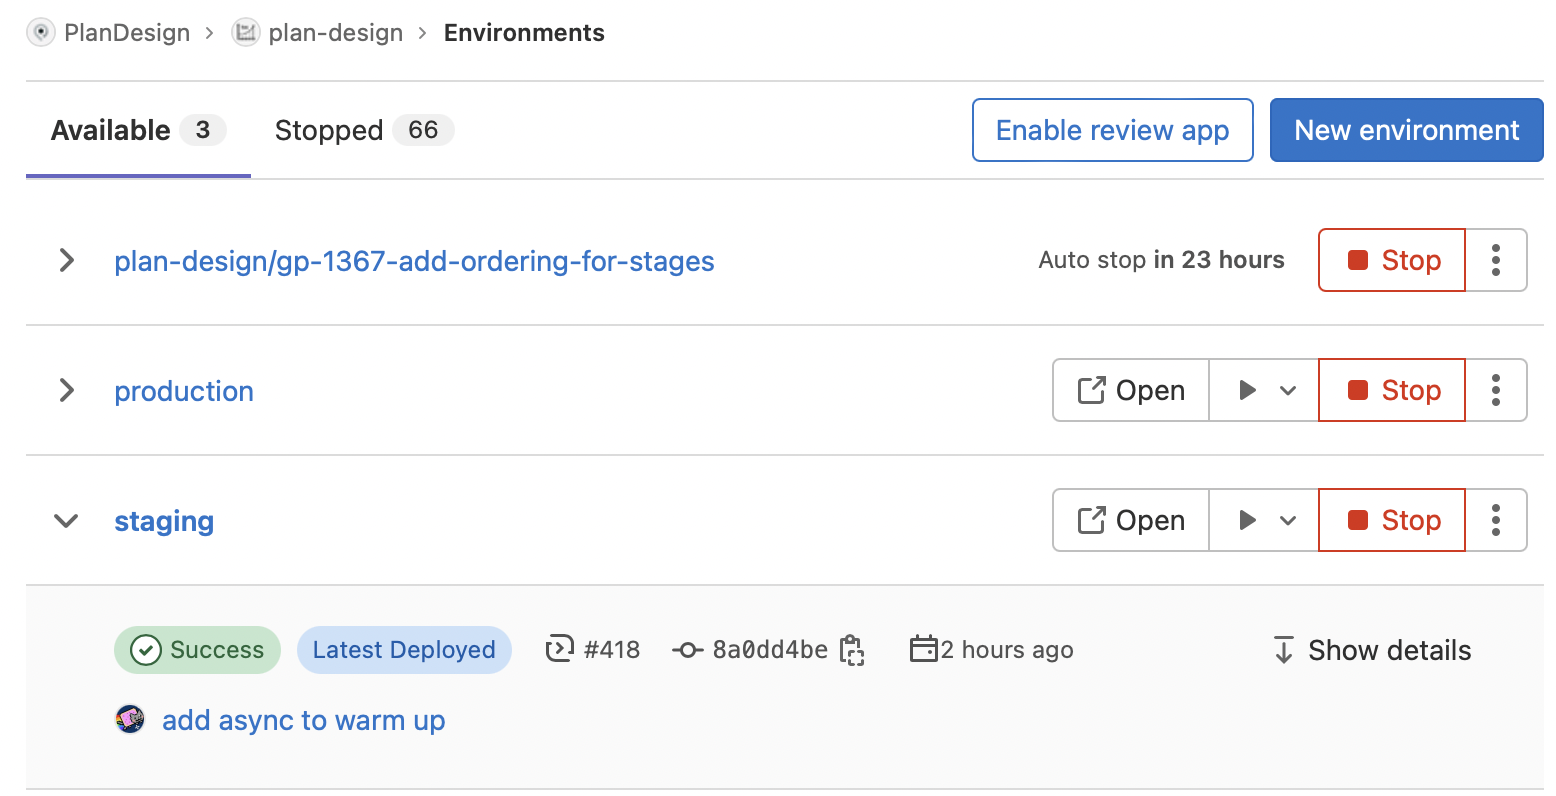
\includegraphics[width=\textwidth]{implementation/pictures/deployment/environment}
	\caption{Пример динамических окружений}
	\label{pic:implementation__deployment-environment}
\end{figure}
\vskip 10 mm

\noindent \textbf{Структура файлов CI/CD}

Все правила развертывания и сборки описываются в файле \textit{.gitlab-ci.yml},
его название и местоположение может быть изменено на любое другое в настройках репозитория.

Сложную конфигурацию CI/CD можно разбить на несколько разных логических компонент, поместив каждую из них
в отдельный файл.
С целью упрощения поддержки и добавления новых правил развертывания предлагается следующая структура файлов.

\dirtree{%
.1 gitlab-ci.
.2 stage1.
.3 services.
.4 service1.yml.
.4 service2.yml.
.4 service3.yml.
.3 main.yml.
.2 stage2.
.3 services.
.4 service1.yml.
.4 service3.yml.
.4 service7.yml.
.3 main.yml.
.2 stage3.
.3 services.
.4 service2.yml.
.4 service3.yml.
.3 main.yml.
.1 main.yml.
}

\vskip 5mm
Данная структура является иерархической.
Корневая директория называется \textit{gitlab-ci}. В корневой директории находится файл
\textit{gitlab-ci/main.yml}
(см. листинг\ref{lst:implementation__deployment_main_yml}),
внутри которого содержатся на верхнеуровневые файлы для каждого \textit{Stage}.
В директории каждого \textit{Stage} находится файл \textit{main.yml} (см. листинг\ref{lst:implementation__deployment_main_stage_yml})
который содержит включения на файлы
с описанием конфигурации для отдельного сервиса на этом этапе.

\lstinputlisting[
    caption={Пример кода \textbf{gitlab-ci/main.yml}},
    captionpos=b,
    label={lst:implementation__deployment_main_yml}
]{implementation/listings/deployment/main.yml}
\vskip 5mm

\lstinputlisting[
    caption={Пример кода \textbf{gitlab-ci/stage1/main.yml}},
    captionpos=b,
    label={lst:implementation__deployment_main_stage_yml}
]
{implementation/listings/deployment/main_stage.yml}
\vskip 5mm
